\documentclass{book}

\usepackage{listings}
\usepackage{theorem}
\usepackage{graphicx}
\usepackage{hyperref}
\usepackage{amsfonts}
\usepackage{amsmath}
\usepackage[table]{xcolor}
\usepackage{array,calc}
\usepackage{amsmath}

\newtheorem{exercise}{Exercise}


\lstset{
  language=Java,
  basicstyle=\ttfamily\footnotesize,
  numbers = left
}

\newcommand{\co}[1]{\lstinline[language=Java, basicstyle=\ttfamily]{#1}}

\begin{document}

\addtocounter{chapter}{5}

\chapter{Transformations}
Common to the point and neighborhood operations discussed so far is the fact that they may change the color of an image, but the position of each pixel and thus the geometry of the image remains the same. The purpose of transformations is to modify an image by moving pixels around. Examples of transformations include rotation, skewing, scaling, rippling and twirling. The application Photo Booth shown below implements a number of image transformations such as bulging, denting, twirling, squeezing, stretching and fish eye.

\begin{center}
\includegraphics[scale=0.5]{photobooth.jpg}\label{img:photobooth}
\end{center}

\section{A Tiny Framework for Transformations}
An image transformation modifies the image by moving pixels around. That is, each pixel in the output image has a corresponding pixel, typically at a different coordinate, in the input image. As such, an image transformation is uniquely determined by how each coordinate in the output image is mapped to a corresponding coordinate in the input image. To model the common aspects shared by all transformations, we define an abstract class \co{Transformation}:
\begin{lstlisting}
public abstract class Transformation {

  public abstract Point pointFunction(Point point);

  public void applyTo(ImageProcessor ip) {
    ImageProcessor copy = ip.duplicate();
    for (int x = 0; x < ip.getWidth(); x++) {
      for (int y = 0; y < ip.getHeight(); y++) {
        Point p = pointFunction(new Point(x, y));
        int newColor = copy.getPixel((int) round(p.x), (int) round(p.y));
        ip.putPixel(x, y, newColor);
      }
    }
  }
}
\end{lstlisting}
The template method \co{applyTo} assigns a new color to each pixel. For each pixel in the output image, the coordinate of the corresponding pixel in the input image is computed by \co{pointFunction}. Coordinates are represented by objects of the class \co{Point}:
\begin{lstlisting}
public class Point {
  final double x, y;

  public Point(float x, float y) {
    this.x = x;
    this.y = y;
  }
}
\end{lstlisting}
Specific image transformations are modelled as subclasses of \co{Transformation}. In particular, subclasses must override the abstract method \co{pointFunction}. For example, the class \co{TranslateRight} shown below moves (or translates) all pixels in the image 100 pixels to the right:
\begin{lstlisting}
public class TranslateRight extends Transformation {

  @Override
  public Point pointFunction(Point point) {
    return new Point(point.x - 100, point.y);
  }
}
\end{lstlisting}
The method \co{pointFunction} answers the question: where does the pixel located at \co{point} in the output image come from? When translating an image 100 pixels to the right, a pixel located at $(x, y)$ in the output image was originally located at $(x - 100, y)$ in the input image. This transformation can be applied to an image as follows:
\begin{lstlisting}
ImageProcessor ip = ...
Transformation transformation = new TranslateRight();
transformation.applyTo(ip);
\end{lstlisting}

\begin{exercise}
Add the classes \co{Transformation}, \co{Point} and \co{TranslateRight} to your Eclipse project. Apply \co{TranslateRight} to \co{lena.png}. What do you expect will happen? Why does the output image contain black pixels on the left?
\end{exercise}

\begin{exercise}
Create a new subclass of \co{Transformation} named \co{Flip} that horizontally flips an image. The output of \texttt{Flip} for \texttt{lena.png} should look as follows:
\begin{center}
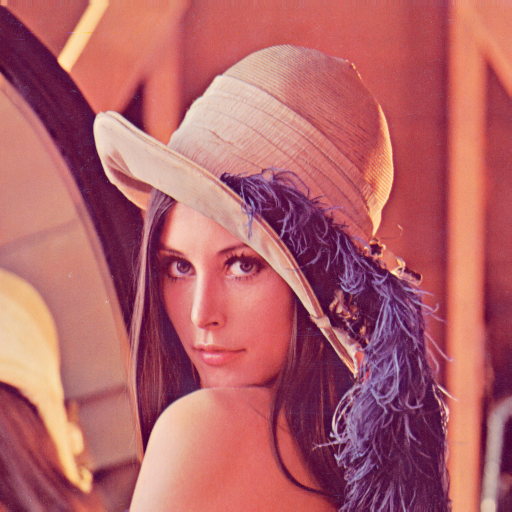
\includegraphics[scale=0.2]{lena-flipped-horizontally.png}
\end{center} 
\end{exercise}

\begin{exercise}
Photo Booth contains a transformation named \emph{Mirror} that mirrors the left half of the image on the right. This transformation is shown the screen shot on page~\pageref{img:photobooth}. Create a new subclass of \co{Transformation} named \co{Mirror} that implements this transformation. The output of \texttt{Mirror} for \texttt{lena.png} should look as follows:
\begin{center}
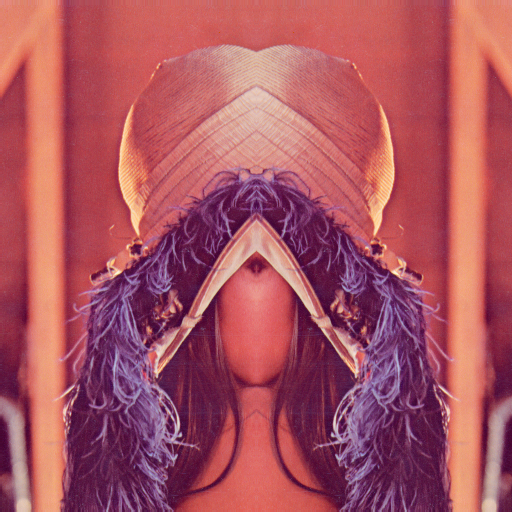
\includegraphics[scale=0.2]{lena-mirror.png}
\end{center} 
\end{exercise}

\begin{exercise}\label{ex:zoom}
Image editing programs typically provide a way to zoom in on an image. For example, Gimp provides this functionality under \co{View>Zoom}:
\begin{center}
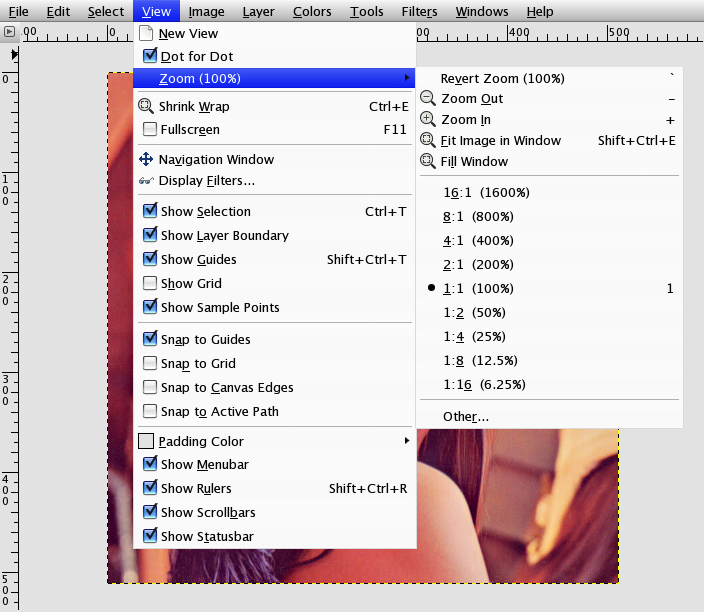
\includegraphics[scale=0.3]{gimp-zoom.png}
\end{center} 
Create a new subclass of \co{Transformation} named \co{Zoom} that enlarges (or zooms in on) the image by a certain factor. The factor is a parameter of \co{Zoom}'s constructor. The output of \texttt{Zoom} for \texttt{lena.png} with factor $2$ should look as follows:
\begin{center}
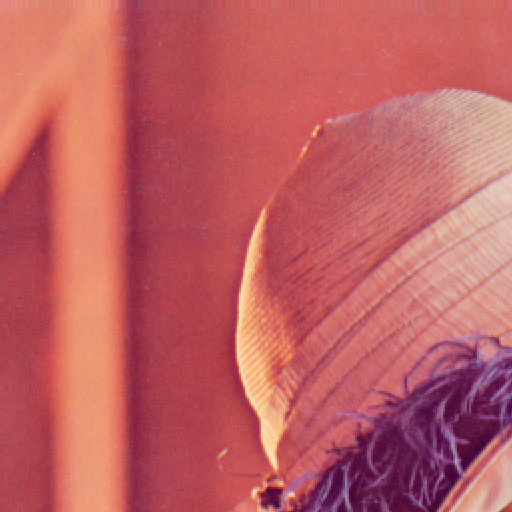
\includegraphics[scale=0.2]{lena-zoom-2.png}
\end{center} 
\end{exercise}

\begin{exercise}\label{ex:zoom-center}
The class \co{Zoom} of exercise~\ref{ex:zoom} zooms in on the upper left corner of the image. Modify this class such that the transformation zooms in on the center of the image. For example, zooming in on the center of \texttt{lena.png} with factor $2$ results in the following image:
\begin{center}
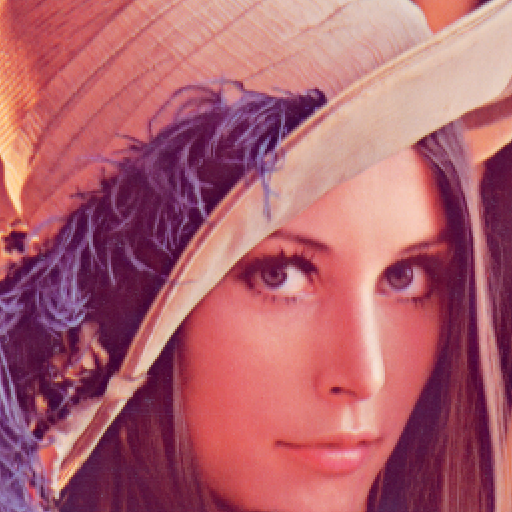
\includegraphics[scale=0.2]{lena-zoom-center-2.png}
\end{center} 
\end{exercise}

\begin{exercise}
Refactor the class \co{Zoom} such that the user can select the coordinate of the pixel that forms the center of the zoom operation.
\end{exercise}

\begin{exercise}
Create a new subclass of \co{Transformation} named \co{Rotate} that rotates an image by a certain angle $\theta$ in clockwise direction around the top left corner. The angle $\theta$ is an argument of the constructor.

As you may remember from the course ``Wiskunde voor Informatici'', rotation is an example of a linear transformation. Each linear transformation on Cartesian coordinates can be captured in a $2\times2$ transformation matrix. The transformation matrix for rotating with an angle $\theta$ in clockwise direction is the following: 
$$T_{rotate} = \begin{bmatrix}
\cos(\theta) & -\sin(\theta)\\
\sin(\theta) & \cos(\theta)\\
\end{bmatrix}$$
Rotating a coordinate $(x, y)$ can then be expressed as a matrix multiplication:
$$
\begin{bmatrix}
x'\\ y'\\ 
\end{bmatrix} = \begin{bmatrix}
\cos(\theta) & -\sin(\theta)\\
\sin(\theta) & \cos(\theta)\\
\end{bmatrix} \cdot \begin{bmatrix}
x\\ y\\
\end{bmatrix}$$
That is, rotating a coordinate $(x, y)$ $\theta$ degrees in clockwise direction results in the coordinate $(\cos(\theta) x - \sin(\theta) y, \sin(\theta) x + \cos(\theta) y)$.

An angle can be measured either in degrees or in radians. For example, $90^{\circ}$ corresponds to $\pi/2$ in radians. Java provides the methods \co{Math.toRadians} and \co{Math.toDegrees} to convert an angle measured in degrees to an equivalent angle measured in radians and vice versa.  $\sin$ and $\cos$ can be computed in Java using the methods \co{Math.sin} and \co{Math.cos}. These methods expect an angle measured in radians.

Rotating \texttt{lena.png} by 20 degrees results in the following image:
\begin{center}
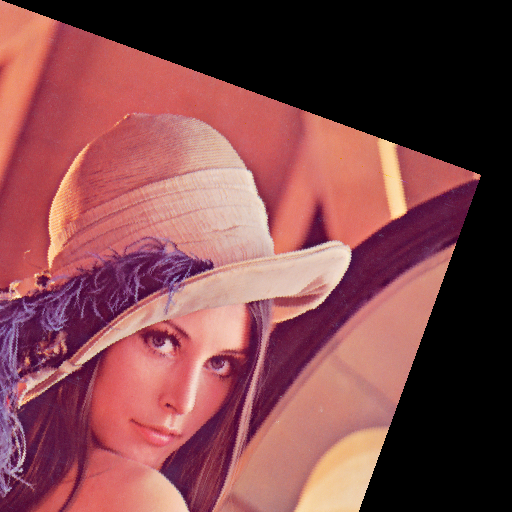
\includegraphics[scale=0.2]{lena-rotated-20.png}
\end{center} 
\end{exercise}

\begin{exercise}
The class \co{Rotate} rotates an image around the top left corner. Modify this class such that the image is rotated around the center. Rotating \texttt{lena.png} by 20 degrees around its center results in the following image:
\begin{center}
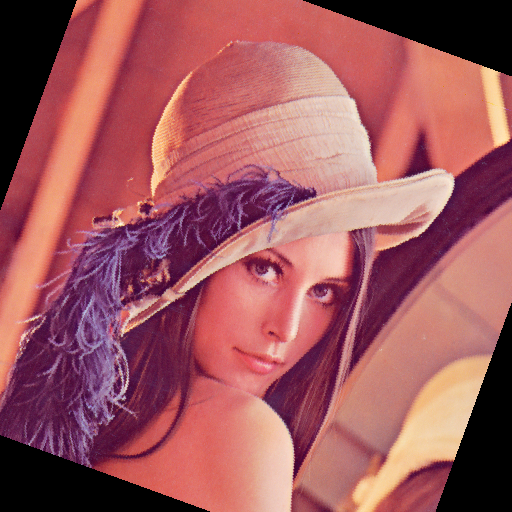
\includegraphics[scale=0.2]{lena-rotated-center-20.png}
\end{center} 
\end{exercise}

\begin{exercise}
As shown on page~\pageref{img:photobooth}, Photo Booth contains a transformation named \emph{Twirl} where each pixel is rotated around the center with an angle that depends on the distance from the center. The transformation takes two arguments: \co{rmax} and \co{thetamax}. The rotation angle decreases linearly starting at \co{thetamax} as the distance from the center increases. The image remains unchanged outside a limiting radius \co{rmax}. Thus, the rotation angle for a pixel at distance $d$ from the center is defined as follows: 
$$angle(d) = \left\{\begin{array}{c l}
  ((\mathtt{rmax} - d)/\mathtt{rmax})*\mathtt{thetamax} & \text{if ${d} < \mathtt{rmax}$}\\
  0 & \text{otherwise}\\
\end{array}
\right.$$
The distance from the center $d$ of a pixel at $(x, y)$ can be computed via the following formula:
$$d=\sqrt{(x - x_c)^2 + (y-y_c)^2}$$
where $(x_c, y_c)$ is the coordinate of the center.

Twirling \texttt{lena.png} with \co{thetamax} equal to $60$ and \co{rmax} equal to $250$ results in the following image:
\begin{center}
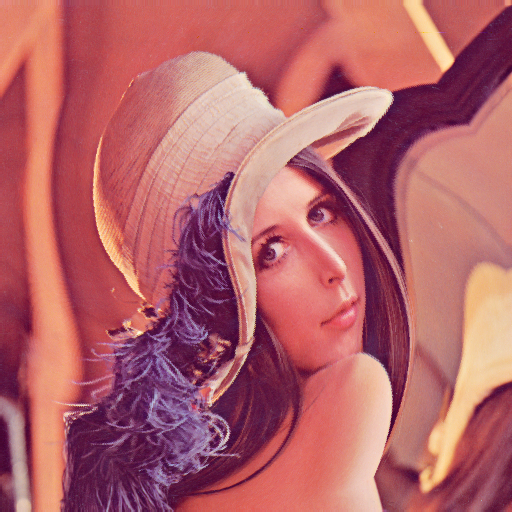
\includegraphics[scale=0.2]{lena-twirled-60.png}
\end{center} 
\end{exercise}

\begin{exercise}
Twirling is an example of a invertible image transformation. This means that the effect of the transformation can be undone by applying the inverse transformation. \co{mysteryperson5.png} was twirled with \co{thetamax} equal to $270$ and \co{rmax} equal to $210$. Who is the famous wizard distorted by the transformation?
\end{exercise}

\begin{exercise}
Gimp provides a rippling filter. This filter can be accessed via the menu item \texttt{Filters>Distorts>Ripple...}.
\begin{center}
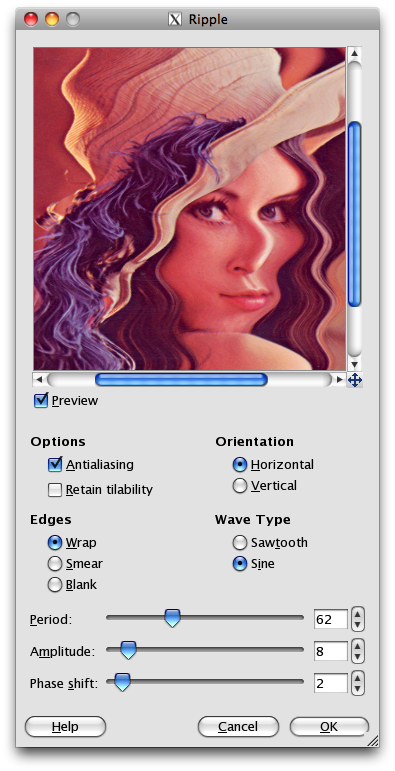
\includegraphics[scale=0.2]{gimp-rippling.png} 
\end{center}
Create a new subclass of \co{Transformation} named \co{Ripple} that implements rippling. This transformation has 3 arguments: an amplitude $a$, a phase $\phi$ and a period length $\tau$. 
$$\begin{array}{c}
x' = x + a \cdot \sin(\frac{2\pi\cdot y}{\tau})\\
y' = y\\
\end{array}$$   
Rippling \texttt{lena.png} with $a=10$, $\tau=100$ and $\phi = 0$ results in the following image:
\begin{center}
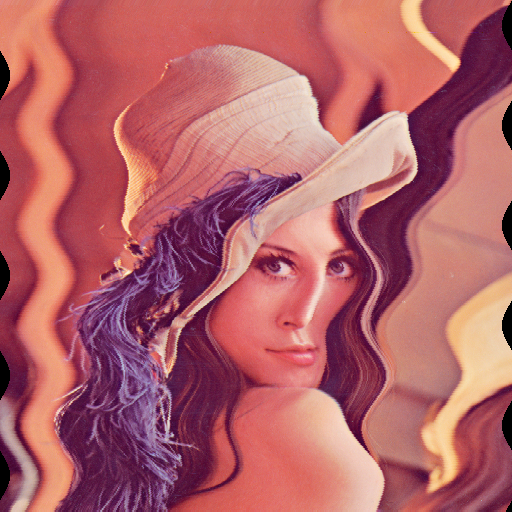
\includegraphics[scale=0.2]{lena-rippled.png}
\end{center}
\end{exercise}

\begin{exercise}
Create a new subclass of \co{Transformation} named \co{Tiling} which subdivides the image into several tiles. Each tile contains a copy of the original image. The width and height of each tile are parameters of \co{Tiling}'s constructor. The images below show the effect of tiling on \texttt{lena.png} where width and height are both equal to respectively 256, 128 and 64.
\begin{center}
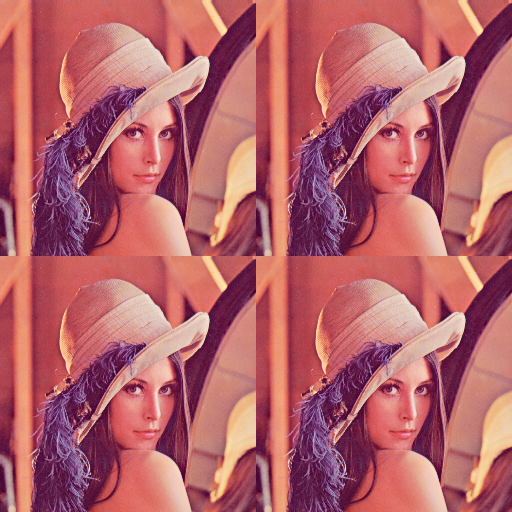
\includegraphics[scale=0.2]{lena-tiled-256.png}
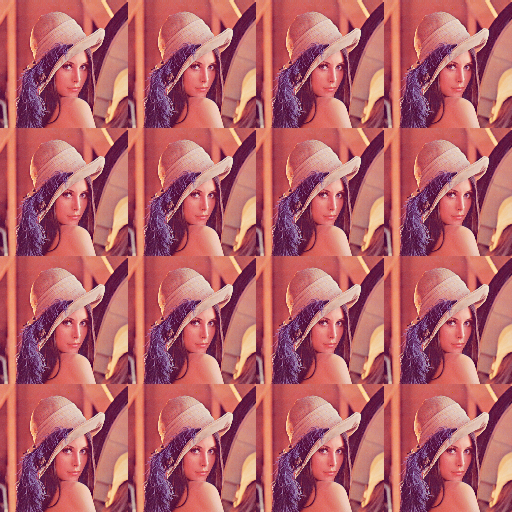
\includegraphics[scale=0.2]{lena-tiled-128.png}
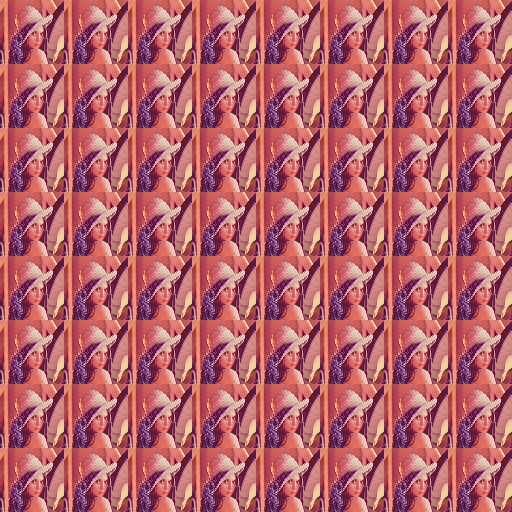
\includegraphics[scale=0.2]{lena-tiled-64.png}
\end{center} 
\end{exercise}

%\begin{exercise}\label{ex:shrink}
%Create a new subclass of \co{Transformation} named \co{Shrink} that shrinks an image by a certain factor. The factor is a parameter of \co{Shrink}'s constructor. The output of \texttt{Shrink} for \texttt{lena.png} with factor $2$ should look as follows:
%\begin{center}
%\includegraphics[scale=0.2]{lena-shrink-2.png}
%\end{center} 
%\end{exercise}

\section{Linear Transformations}


%composing transformations

% interpolation
% zooming in: aliasing

\end{document}